\documentclass{report}
\def\atitle{Development of a Control System Using a Raspberry Pi}
\def\theauthor{Christopher Boyle}

% Imports
\usepackage{graphicx}
\usepackage[a4paper]{geometry}
\usepackage{fancyhdr}
\usepackage[english]{babel}
\usepackage{etoolbox}
\usepackage{url}
\usepackage[hidelinks]{hyperref}

% Unused packages
%\usepackage{placeins}
%\usepackage{fancyref}
%\usepackage[comma,authoryear]{natbib}
%\usepackage{lipsum}

% Settings
\geometry{top=2cm, bottom=2cm, left=0cm, right=0cm}
\patchcmd{\chapter}{\thispagestyle{plain}}{\thispagestyle{plain}}{}{}
\setcounter{secnumdepth}{0}
\renewcommand{\theequation}{\thetitle.\arabic{equation}}
\renewcommand\UrlFont{\rmfamily\itshape}

% Header/footer preamble
\fancyhf{}
\fancypagestyle{plain}{
	\renewcommand{\headrulewidth}{0.4pt}
	\renewcommand{\footrulewidth}{0.4pt}
	\fancyhead[L]{\atitle}
	\fancyhead[R]{\theauthor}
	\fancyfoot[L]{\today}
	\fancyfoot[R]{\thepage}
}
\begin{document}

	\begin{titlepage}
		\newgeometry{top=2cm, bottom=2cm, left=3cm, right=3cm}
		\makebox[\textwidth][c]{
\includegraphics[scale=1]{images/titleheader.png}}
		\centering
		\vskip4cm
		{
			\bfseries\Large
			Department of Chemical \& Process Engineering\\
			\vskip1cm
			MEng in Chemical \& Process Engineering\\
			18530
			\vskip3cm
			\LARGE\atitle
		}
		\vskip3cm
		{\small Word Count: 10,000}
		\vskip1cm
		\begin{flushleft}
			This project is submitted in partial fulfillment of the regulations governing the award of \\
			Degree of MEng in Chemical Engineering at the University of Strathclyde
			\vskip2cm
			Your name: Christopher Boyle \hfill Date: \today
			\vskip1cm
			Organisation: University of Strathclyde, Department of Chemical \& Process Engineering\newline% \newline
			In-house Supervisor: Dr. Leo Lue \newline% \newline
			Academic Supervisor: Dr. Leo Lue
		\end{flushleft}
	\end{titlepage}

	% Main Content Settings
	\newgeometry{top=2cm, bottom=2cm, left=3cm, right=3cm}
	\pagenumbering{roman}
	
	% Summary Page
	\chapter*{Summary}
	\addcontentsline{toc}{chapter}{Summary}
	%Brief, factual, generally following the same order of presentation as the report. Do not include figures, tables, or references.
	
	% Contents Page
	\tableofcontents
	
	% Acknowledgements
	\chapter*{Acknowledgements}
	\addcontentsline{toc}{chapter}{Acknowledgements}
	%It is a matter of honesty and courtesy that acknowledgement is made to those who helped you in your work.
	%Dr. Lue
	
	\newpage
	\pagenumbering{arabic}
	\setcounter{page}{1}
	
	\chapter*{Introduction}
	\addcontentsline{toc}{chapter}{Introduction}
	%The introduction sets the scene. It should include a brief description of the organisation, the type of work carried out, projects undertaken, background information to the work carried out and a brief outline of the report and of the learning objectives for the project.
	%History of what is being done, what is used to do it, how it is done.



	\section{Laboratory Automation}
	Laboratory automation involves the design and implementation of robotic systems which are able to conduct laboratory experiments automatically, reducing the workload of human scientists and technicians \cite{backwhatisauto}. This includes the use of machine learning and AI to interpret results and create hypotheses \cite{backlitrevai, backbaconauto, backlabauto}. The motivation for this is eaasy to see, "Robot Scientists" can be used to conduct experiments with little to no human supervision and can take in a vast number of measurements. The "Adam" Robot Scientist developed by the team at Aberystwyth University can make over 200,000 measurements a day (moreover, it can make over 1,000,000 other observations and hypothoses per day)  \cite{backontorobsci}.\newline \newline \noindent
	%More history?
	Laboratory automation is similar in concept to process control (EXPLAIN). Electronic process controllers make use of small computers called microcontrollers to calculate their response to changing process conditions \cite{backprocautotheory}. A microcontroller chip is a small user-programmable "computer" which reads input from, and outputs data to an electronic circuit in order to achieve the overall objective \cite{backwhatismc}. A desktop computer consists, basically, of a processor, memory, and storage, microcontrollers are composed of the same components but contained within a single package (see Figure \ref{mcudia}). Microcontrollers are programmed by connecting them to a "master" computer which can set the data on the microcontroller's storage. Data is stored as binary data (data is stored solely in the form of 0s and 1s). The program is written in a programming language, a special set of instructions which the environment can understand and convert into actions (like saving a value to memory). For further discussion on programming languages see Appendix 1.
	\begin{figure}[h!]
	\centering
	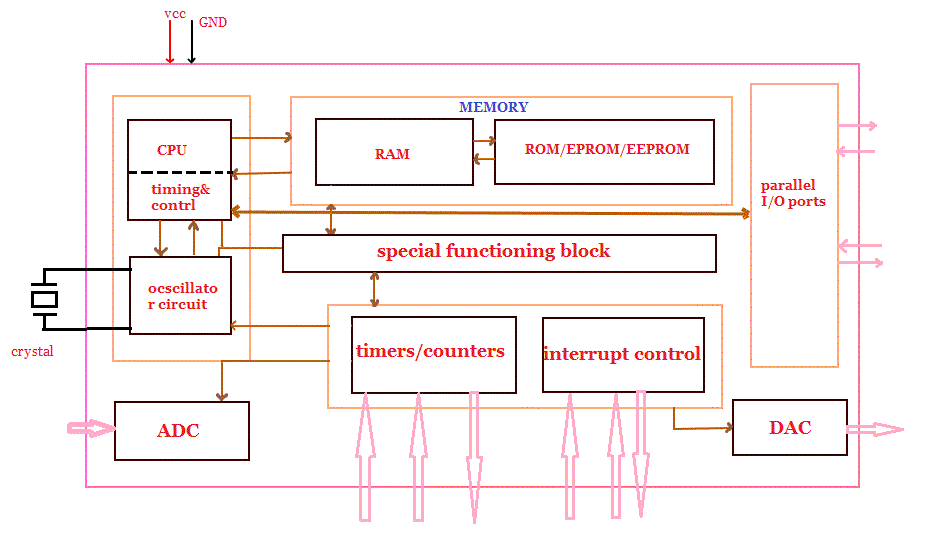
\includegraphics[scale=0.5]{images/mcudia.png}
	\caption{Microcontroller Block Diagram (taken from  \cite{mcudia})}
	\label{mcudia}
	\end{figure}



	\section{Raspberry Pi}
	\noindent
	Microcontrollers are commonly used in education to teach computer programming \cite{backmcedu1, backmcedu2}. However, it was noticed that people were not fully learning about how computers work in schools and universities and so the Raspberry Pi Foundation was founded, and the Raspberry Pi Model A was developed as a platform to facilitate eduction \cite{pihistory}. The Raspberry Pi is a small (85mm x56mm) \cite{pi3mechdraw} computer running a version ("flavour") of GNU/Linux called "Raspian" by default (it is able to run a number of other operating systems if desired \cite{piotheros}).  \newline
	\begin{figure}[h!]
	\centering
	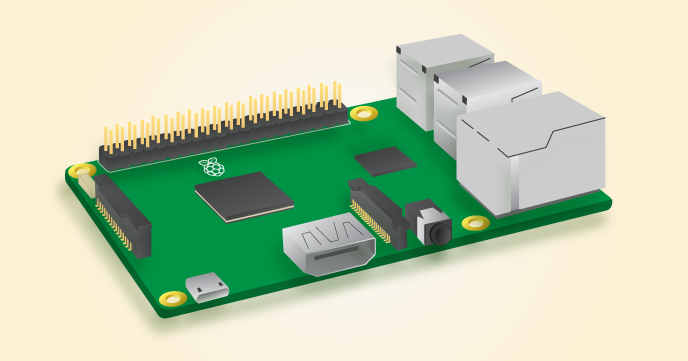
\includegraphics[scale=0.5]{images/pi3modelb.png}
	\caption{Raspberry Pi 3 Model B (taken from  \cite{pi3info})}
	\label{pidia}
	\footnotesize Clockwise from top left: GPIO pins, USB ports, Ethernet port, audio jack, Camera Serial Interface (CSI), HDMI port, micro-USB power port, and Display Serial Interface (DSI).
	\end{figure} \newline \noindent
	The first Raspberry Pi (Model A) had a single core 700MHz processor and 256MB of RMA \cite{pi1info}, while the current Raspberry Pi 3 Model B has a quad core 1.2GHz and 1GB of RAM (also including built in WiFi and Bluetooth) \cite{pi3info}. The quad core processor enables better multithreaded operation for software running on the Raspberry Pi, meaning that big cumbersome programs can run much more efficiently than before. In addition, the increase in memory and CPU clock frequency means there is overall a massive performance boost. Operations like compiling a large program (for example OpenCV, the Open Source Computer Vision Library) which would take over 9 hours \cite{pipowercompold} on the Raspberry Pi 1, takes little over an hour and a half \cite{pipowercompnew} on the lastest model.\newline \newline  \noindent
	Despite being initially designed for educational purposes, the Raspberry Pi has found success in other areas such as with hobbyists \cite{pihobbynotedu} and in industry \cite{pimorethanedu}.\newline \newline  \noindent
	What makes the Raspberry Pi interesting to industry, are the GPIO (General Purpose Input/Output, see Figure \ref{pidia}) pins made available on the main board. These pins allow electronic circuits to interface with the Raspberry Pi, and allows software to interact with the real world in a way that is not as easy to accomplish with a tradition computer. This marriage of microcontroller and desktop computer allows for incredibly easy development and testing in a single package. In addition to this, the Raspberry Pi retails (at the time of writing) for £30.00 \cite{picost} making it a very cost effective alternative to other control solutions (which can cost several hundred pounds \cite{otherpcucost}). Each of the GPIO pins is numbered so that they can be referenced, and some have specific purposes other than general purpose input/output (see Figure \ref{gpiopinout})\newline
	\begin{figure}[!h]
	\centering
	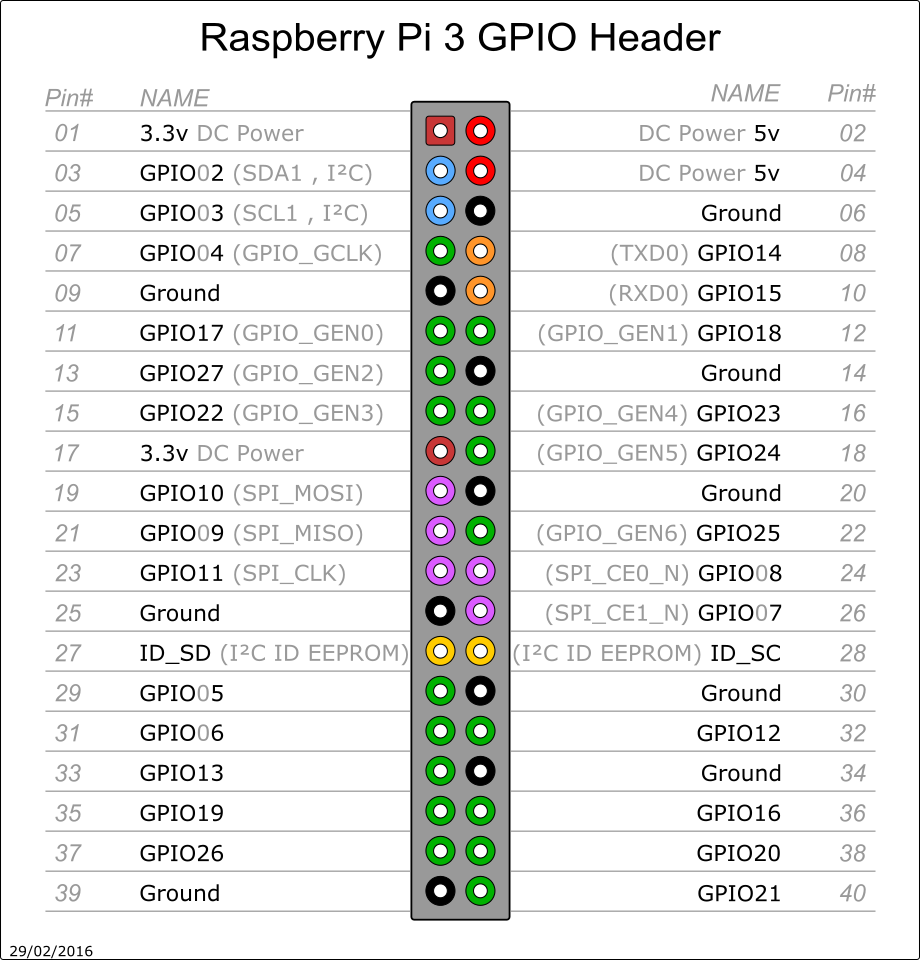
\includegraphics[scale=0.2]{images/gpiopinout.png}
	\caption{Raspberry Pi 3 Model B GPIO Pinout Diagram (taken from  \cite{pigpiopinout})}
	\label{gpiopinout}
	\end{figure} \newline  \noindent
	In addition to simple GPIO functionality, some of the Raspberry Pi's GPIO pins have special functionality. Pins 3 and 5 can also be used to communicate with integrated circuits with the \(I^2 C\) protocol (Inter-Integrated Circuit). This allows bytes of data to be sent over only two wires (CITE I2C). This is done by \textit{serial communication}. Serial communication is where each bit of data (starting with the most significant bit, the highest value bit) is sent one after the other down a wire (CITE SERIAL COMMUNICATION). Another wire is used to synchronise the communication beteween devices. The \(I^2 C\) protocol allows multiple devices to be connected together (termed "daisy-chaining") using the same wires, significantly saving space (CITE I2C DAISY CHAIN). Pins 19, 21, 23, 24, and 26 are used for another serial communications protocol, the Serial Peripherial Interface (SPI) protocol (CITE SPI). Serial communication makes inter device communication much easier. To send the number 1750 to an integrated circuit, the Raspberry Pi would need at least 11 free GPIO pins. While this is not impossible, the number of GPIO pins taken up by the single device is extremely inconvenient. This can easily be sent via serial connection with just two wires.\newline \newline  \noindent
	The high level languages used to create programs on desktop computers can be similarly used to write programs on the Raspberry Pi (it is running a desktop operating system). There are a number of libraries (collections of software) available for facilitating the communication between the software and the GPIO pins. Built in to the Raspberry Pi are some basic languages offering simple functionality, but there are third-party libraries available for anyone to download and use\cite{pilibswiringpi, pilibspigpio}. The programming language "Python" is popular amoungst Raspberry Pi software developers. Python is a high level, object oriented, interpreted language, making it well suited to quickly developing clean, and easy to use object-oriented software. Due to its popularity, Python has a vast number of packages available to perform any number of functions.



	\section{This Project}
	Colloidal suspensions are a multiphase mixture consisting of solid particles of a particular size (specifically, WHAT) (CITE) dispersed in a liquid. These mixtures exhibit interesting rheological properties. "Normal" fuids (like water) exhibit Newtonian behaviour - they are viscous (CITE). This means that the rate of shear (how fast they deform) is directly proportional to the shear stress imposed upon them, with the constant of proportionality being the inverse of the viscosity of the fluid. This means that the higher the viscosity of a fluid, the more resistant to deformation the fluid is. Multiphase suspensions can exhibit non-Newtonian behaviour, where this direct relationship is not found. Some exhibit a shear-thickening behaviour: as the shear stress is increased, the shear rate decreases faster than in newtonian behaviour (CITE). Others exhibit shear thinning. Figure \ref{nonnewtgraphs} shows how shear rate varies with shear stress for select non-newtonian fluids. The phenomenom of "jamming" is where a multiphase suspension undergoing shear, has a sudden decrease in shear rate. This can cause problems (LIKE) (CITE). \newline
	\begin{figure}[!h]
	\centering
	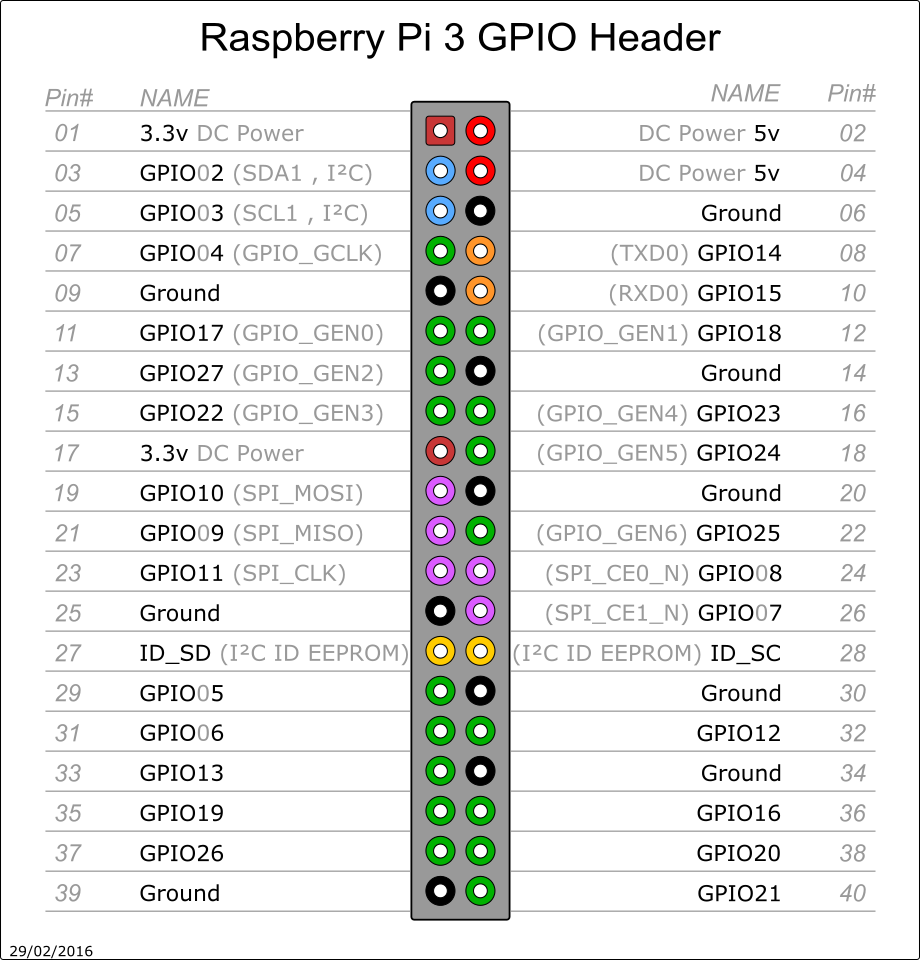
\includegraphics[scale=0.2]{images/gpiopinout.png}
	\caption{DO ME (taken from (CITE))}
	\label{nonnewtgraphs}
	\end{figure} \newline  \noindent
	This project aims to design, build, and test a control system for an experimental set up revolving around gathering more information about the occurance of the "jamming" phenomenon. The experimental process consists of two concentric cylinders, the inner of which is attached to a DC motor and can be rotated. The gap between the two cylinders will be filled with a colloidal suspension. A piezoelectric crystal with a needle (the PiezoElectric Needle Device, PEND) attached will be held above the cylinders such that the tip of the needle is just touching the surface of the fluid (SEE FIGURE (ALSO, DRAW FIGURE)). (Camera, other stuff) \newline \newline \noindent
	The motor's rotational speed will be set at different values and will have to be controlled to ensure it is maintained. The PEND can be used to detect the torque imposed upon the fluid (and thus the shear stress) by recording the potential difference accross the crystal as the needle is deflected by the moving fluid and thus distorts the piezoelectric crystal.  \newline \newline \noindent
	The Raspberry Pi's low cost, low power consumption, and GPIO availability make it a suitable choice for the controller to this process. Software will be developed for the Raspberry Pi to read in the motor's speed and the PEND's voltage reading, record it accurately and to control the rotational speed of the motor. In addition, the Raspberry Pi can be used to automate the experimental process by automatically completing runs and altering experimental parameters. The Pi can also be set up with a web interface, allowing monitoring of the experiment from remote locations, further reducing the manual workload on lab technicians.

	%\chapter*{Description of the Organisation}
	%\addcontentsline{toc}{chapter}{Description of the Organisation}
	%In this section, you should show a good understanding of the organisation. Details may include the type of organisation, management structure, products, and markets catered for. Mention your position in the organisation.
	
	\chapter*{Description of the Work}
	\addcontentsline{toc}{chapter}{Description of the Work}
	%Elaborate on issues mentioned in introduction. Use a logical development, not necessarily in chronological order. Explain the significance, purpose and nature of your work. Describe methods used and outcomes. Try to ensure a balanced treatment of issues, in accordance with their relative importance, and excluding irrelevant material. Present results and discuss around them. Explain the significance of these results and their impact on the organisation. Comment on technical difficulties you may have experienced. In a long report, subdivide with appropriate sub-headings, or divide this section into different sections. Equations should be numbered sequentially (see templates document).
	\section{Experimental Setup}
	\section{Electronic Circuits}
	\section{Software}
	\section{Procedure}
	\chapter*{Conclusions}
	\addcontentsline{toc}{chapter}{Conclusions}
	%Summarise findings and inferences mentioned in the core of the report. Try to be as brief as possible, with concise statements. Include recommendations, where appropriate. 
	
	\chapter*{Review}
	\addcontentsline{toc}{chapter}{Review}
	%Relate this section to the learning objectives in the introduction. Report what you have learnt about the organisation and about yourself. Mention your achievements, what you have learnt, skills you have acquired or improved. This might be technical or "soft" skills. Try to relate this to what you have learned in your coursework at University and what skills you will take forward to your first full time professional post.
	
	\chapter*{Nomenclature}
	\addcontentsline{toc}{chapter}{Nomenclature}
	%List all the symbols in alphabetical order, with Greek symbols at the end.
	\begin{center}
		\begin{tabular}{|c|c|}
			\hline
			\rule{3cm}{0pt}\textbf{Symbol}\rule{3cm}{0pt} & \rule{3cm}{0pt}\textbf{Description}\rule{3cm}{0pt} \\
			\hline
			 & \\
			\hline
			& \\
			\hline
			& \\
			\hline
			& \\
			\hline
			& \\
			\hline
			& \\
			\hline
			& \\
			\hline
			& \\
			\hline
		\end{tabular}
	\end{center}
	
	%Main Bibliography

	\addcontentsline{toc}{chapter}{Bibliography}
	\bibliography{biblio}
	\bibliographystyle{unsrt}

%Appendix

\chapter*{Appendices}
\addcontentsline{toc}{chapter}{Appendices}
\pagenumbering{alph}
\setcounter{page}{1}
\setcounter{section}{1}
\section{Appendix 1 -  Programming Languages}
Programming languages come in many forms. High level languages (like C, Java, C\#, Python) are abstracted from the binary in which it will be eventually stored. High level languages consist of a natural-like language which is converted by a "compiler" or "interpreter" into machine code, understandable by the processor.\newline \newline  \noindent
\noindent
An example of a high level language (Python):
\begin{verbatim}
                    from time import time()

                    alarm_time = 2147483647

                    while (time() != alarm_time):
                              pass

                    print("Alert!")
\end{verbatim}
An example of a machine code (in hexadecimal)\cite{proglangmachex}:
\begin{verbatim}
                    0x 60 00 00 80
                    0x A4 00 00 00
                    0x 60 01 00 84
                    0x A4 01 01 00
                    0x 60 02 00 00
                    0x 60 03 00 04
                    0x 60 04 00 00
                    0x 60 05 00 01
                    0x 08 00 00 02
                    0x 20 00 00 03
                    0x 20 04 04 05
                    0x 11 20 04 01
\end{verbatim}
	From the above it can be seen that high level languages, while not strictly English, are far easier to read than machine code. Machine code will take multiple instructions to achieve the same thing that could be done in a single line in a high level language, thus a high level instruction needs to be converted into multiple machine level instructions for the processor to understand it. There are different ways of doing this, leading to diversity in the types of high level languages. (MISSING LINK). Object Oriented Programming Languages (OOPLs) deal with data in terms of "objects"\cite{proglangwhatisoopl}. An object is, like the name suggest, something. This something has properties, and can have things done to it. In the above Python example, "alarm\_time" is a number object, and it is being assigned a value. A "method" is a way of doing something in the program. In the above, the "time()" method is used to get the current time (in number of seconds since 1 January 1970). The advantage of OOPLs lies in the ability to collect objects and methods together in a class. The "time" class above contains a lot of methods which can be used by the programmer, in the example the "time.time()" method is called from the class. The programmer can therefore define a set of methods for dealing with some data in a certain way in a class, and then create multiple instances of this class with different starting data to make use of different starting data. For example, a "sphere" class could be written, with methods which provide the sphere's surface area and volume, given the sphere's diameter. Then a program could be written to create three sphere class instances, each with different diameters and then the areas and volumes could be calculate simply when needed. This creates tidy programs, which are easier to understand and reduces the amount of redundant code that needs to be written.\newline \newline  \noindent
	Another, less common, type of programming language is the procedural language. This language is simply one instruction following another\cite{proglangwhatisoopl}. The procedural program starts at the start and continues down the list of instructions until it finishes. This language requires writing out the same code multiple times to achieve the same effect as an OOPL, which is a reason for its reduced popularity.\newline \newline  \noindent
	As previously mentioned, code written in a programming language is usually compiled before it is run. However, some languages do not need to be compiled before being run. These languages are called "interpreted" languages and they are "compiled" line by line when you run them \cite{proglanginterp}. Since interpreted languages do not need to be compiled (and so software developers do not have to wait for the compilation step to complete before testing) they are preferred for developing software. However, they tend to run slower than compiled programs for the same reason.\newline \newline  \noindent
	To conclude this section,  programming languages are varied and have different advantages and disadvantages. The correct programming language must be chosen for the correct situation.\newline \newline  \noindent
\section{Appendix 2 -  Alternative Programming Language}
\section{Appendix 3 -  Alternative Controller}
\section{Appendix 4 -  Alternative Operating System}
\section{Appendix 5 -  Alternative Speed Detection Circuit: \newline Hall Effect Sensor}
\section{Appendix 6 -  Alternative Speed Detection Circuit: \newline Dynamo}
\section{Appendix 7 -  Alternative Speed Control Circuit: \newline Digitally Programmable Voltage Regulator}
%Appendix Bibliography

\end{document}